\documentclass[11pt,a4paper,oneside]{report}             % Single-side
%\documentclass[11pt,a4paper,twoside,openright]{report}  % Duplex

%\PassOptionsToPackage{chapternumber=Huordinal}{magyar.ldf}
\usepackage{t1enc}
\usepackage[latin2]{inputenc}
\usepackage{amsmath}
\usepackage{amssymb}
\usepackage{enumerate}
\usepackage[thmmarks]{ntheorem}
\usepackage{graphics}
\usepackage{epsfig}
\usepackage{listings}
\usepackage{color}
%\usepackage{fancyhdr}
\usepackage{lastpage}
\usepackage{anysize}
\usepackage[magyar]{babel}
\usepackage{sectsty}
\usepackage{setspace}  % Ettol a tablazatok, abrak, labjegyzetek maradnak 1-es sorkozzel!
\usepackage[hang]{caption}
\usepackage{hyperref}

%--------------------------------------------------------------------------------------
% Main variables
%--------------------------------------------------------------------------------------
\newcommand{\vikszerzo}{B�dis-Szomor� Andr�s}
\newcommand{\vikkonzulens}{dr.~Konzulens Elem�r}
\newcommand{\vikcim}{Elektronikus terel�k}
\newcommand{\viktanszek}{M�r�stechnika �s Inform�ci�s Rendszerek Tansz�k}
\newcommand{\vikdoktipus}{Diplomaterv}
\newcommand{\vikdepartmentr}{B�dis-Szomor� Andr�s}

%--------------------------------------------------------------------------------------
% Page layout setup
%--------------------------------------------------------------------------------------
% we need to redefine the pagestyle plain
% another possibility is to use the body of this command without \fancypagestyle
% and use \pagestyle{fancy} but in that case the special pages
% (like the ToC, the References, and the Chapter pages)remain in plane style

\pagestyle{plain}
%\setlength{\parindent}{0pt} % �ttekinthet�bb, angol nyelv� dokumentumokban jellemz�
%\setlength{\parskip}{8pt plus 3pt minus 3pt} % �ttekinthet�bb, angol nyelv� dokumentumokban jellemz�
\setlength{\parindent}{12pt} % magyar nyelv� dokumentumokban jellemz�
\setlength{\parskip}{0pt}    % magyar nyelv� dokumentumokban jellemz�

\marginsize{35mm}{25mm}{15mm}{15mm} % anysize package
\setcounter{secnumdepth}{0}
\sectionfont{\large\upshape\bfseries}
\setcounter{secnumdepth}{2}
\singlespacing
\frenchspacing

%--------------------------------------------------------------------------------------
%	Setup hyperref package
%--------------------------------------------------------------------------------------
\hypersetup{
    bookmarks=true,            % show bookmarks bar?
    unicode=false,             % non-Latin characters in Acrobat�s bookmarks
    pdftitle={\vikcim},        % title
    pdfauthor={\vikszerzo},    % author
    pdfsubject={\vikdoktipus}, % subject of the document
    pdfcreator={\vikszerzo},   % creator of the document
    pdfproducer={Producer},    % producer of the document
    pdfkeywords={keywords},    % list of keywords
    pdfnewwindow=true,         % links in new window
    colorlinks=true,           % false: boxed links; true: colored links
    linkcolor=black,           % color of internal links
    citecolor=black,           % color of links to bibliography
    filecolor=black,           % color of file links
    urlcolor=black             % color of external links
}

%--------------------------------------------------------------------------------------
% Set up listings
%--------------------------------------------------------------------------------------
\lstset{
	basicstyle=\scriptsize\ttfamily, % print whole listing small
	keywordstyle=\color{black}\bfseries\underbar, % underlined bold black keywords
	identifierstyle=, 					% nothing happens
	commentstyle=\color{white}, % white comments
	stringstyle=\scriptsize\sffamily, 			% typewriter type for strings
	showstringspaces=false,     % no special string spaces
	aboveskip=3pt,
	belowskip=3pt,
	columns=fixed,
	backgroundcolor=\color{lightgray},
} 		
\def\lstlistingname{lista}	

%--------------------------------------------------------------------------------------
%	Some new commands and declarations
%--------------------------------------------------------------------------------------
\newcommand{\code}[1]{{\upshape\ttfamily\scriptsize\indent #1}}

% define references
\newcommand{\figref}[1]{\ref{fig:#1}.}
\renewcommand{\eqref}[1]{(\ref{eq:#1})}
\newcommand{\listref}[1]{\ref{listing:#1}.}
\newcommand{\sectref}[1]{\ref{sect:#1}}
\newcommand{\tabref}[1]{\ref{tab:#1}.}

\DeclareMathOperator*{\argmax}{arg\,max}
%\DeclareMathOperator*[1]{\floor}{arg\,max}
\DeclareMathOperator{\sign}{sgn}
\DeclareMathOperator{\rot}{rot}
\definecolor{lightgray}{rgb}{0.95,0.95,0.95}

\author{\vikszerzo}
\title{\viktitle}
\includeonly{
	guideline,%
	project,%
	titlepage,%
	declaration,%
	abstract,%
	introduction,%
	chapter1,%
	chapter2,%
	chapter3,%
	acknowledgement,%
	appendices,%
}
%--------------------------------------------------------------------------------------
%	Setup captions
%--------------------------------------------------------------------------------------
\captionsetup[figure]{
%labelsep=none,
%font={footnotesize,it},
%justification=justified,
width=.75\textwidth,
aboveskip=10pt}

\renewcommand{\captionlabelfont}{\small\bf}
\renewcommand{\captionfont}{\footnotesize\it}

%--------------------------------------------------------------------------------------
% Table of contents and the main text
%--------------------------------------------------------------------------------------
\begin{document}
\singlespacing
%--------------------------------------------------------------------------------------
% Rovid formai es tartalmi tajekoztato
%--------------------------------------------------------------------------------------

\footnotesize
\begin{center}
\large
\textbf{\Large �ltal�nos inform�ci�k, a diplomaterv szerkezete}\\
\end{center}

A diplomaterv szerkezete a BME Villamosm�rn�ki �s Informatikai Kar�n:
\begin{enumerate}
\item	Diplomaterv feladatki�r�s
\item	C�moldal
\item	Tartalomjegyz�k
\item	A diplomatervez� nyilatkozata az �n�ll� munk�r�l �s az elektronikus adatok kezel�s�r�l
\item	Tartalmi �sszefoglal� magyarul �s angolul
\item	Bevezet�s: a feladat �rtelmez�se, a tervez�s c�lja, a feladat indokolts�ga, a diplomaterv fel�p�t�s�nek r�vid �sszefoglal�sa
\item	A feladatki�r�s pontos�t�sa �s r�szletes elemz�se
\item	El�zm�nyek (irodalomkutat�s, hasonl� alkot�sok), az ezekb�l levonhat� k�vetkeztet�sek
\item	A tervez�s r�szletes le�r�sa, a d�nt�si lehet�s�gek �rt�kel�se �s a v�lasztott megold�sok indokl�sa
\item	A megtervezett m�szaki alkot�s �rt�kel�se, kritikai elemz�se, tov�bbfejleszt�si lehet�s�gek
\item	Esetleges k�sz�netnyilv�n�t�sok
\item	R�szletes �s pontos irodalomjegyz�k
\item	F�ggel�k(ek)
\end{enumerate}

Felhaszn�lhat� a k�vetkez� oldalt�l kezd�d� \LaTeX-Diplomaterv sablon dokumentum tartalma. 

A diplomaterv szabv�nyos m�ret� A4-es lapokra ker�lj�n. Az oldalak t�k�rmarg�val k�sz�ljenek (mindenhol 2.5cm, baloldalon 1cm-es k�t�ssel). Az alap�rtelmezett bet�k�szlet a 12 pontos Times New Roman, m�sfeles sork�zzel.

Minden oldalon - az els� n�gy szerkezeti elem kiv�tel�vel - szerepelnie kell az oldalsz�mnak.

A fejezeteket decim�lis beoszt�ssal kell ell�tni. Az �br�kat a megfelel� helyre be kell illeszteni, fejezetenk�nt decim�lis sz�mmal �s kifejez� c�mmel kell ell�tni. A fejezeteket decim�lis al�oszt�ssal sz�mozzuk, maxim�lisan 3 al�oszt�s m�lys�gben (pl. 2.3.4.1.). Az �br�kat, t�bl�zatokat �s k�pleteket c�lszer� fejezetenk�nt k�l�n sz�mozni (pl. 2.4. �bra, 4.2 t�bl�zat vagy k�pletn�l (3.2)). A fejezetc�meket igaz�tsuk balra, a norm�l sz�vegn�l viszont haszn�ljunk sorkiegyenl�t�st. Az �br�kat, t�bl�zatokat �s a hozz�juk tartoz� c�met igaz�tsuk k�z�pre. A c�m a jel�lt r�sz alatt helyezkedjen el.

A k�peket lehet�leg rajzol� programmal k�sz�ts�k el, az egyenleteket egyenlet-szerkeszt� seg�ts�g�vel �rj�k le (A \LaTeX~ehhez k�zenfekv� megold�sokat ny�jt).

Az irodalomjegyz�k sz�vegk�zi hivatkoz�sa t�rt�nhet a Harvard-rendszerben (a szerz� �s az �vsz�m megad�s�val) vagy sorsz�mozva. A teljes lista n�vsor szerinti sorrendben a sz�veg v�g�n szerepeljen (sorsz�mozott irodalmi hivatkoz�sok eset�n hivatkoz�si sorrendben). A szakirodalmi forr�sok c�meit azonban mindig az eredeti nyelven kell megadni, esetleg z�r�jelben a ford�t�ssal. A list�ban szerepl� valamennyi publik�ci�ra hivatkozni kell a sz�vegben (a \LaTeX-sablon a Bib\TeX~seg�ts�g�vel mindezt automatikusan kezeli). Minden publik�ci� a szerz�k ut�n a k�vetkez� adatok szerepelnek: foly�irat cikkekn�l a pontos c�m, a foly�irat c�me, �vfolyam, sz�m, oldalsz�m t�l-ig. A foly�irat c�meket csak akkor r�vid�ts�k, ha azok nagyon k�zismertek vagy nagyon hossz�ak. Internet hivatkoz�sok megad�sakor fontos, hogy az el�r�si �t el�tt megadjuk az oldal tulajdonos�t �s tartalm�t (mivel a link egy id� ut�n ak�r el�rhetetlenn� is v�lhat), valamint az el�r�s id�pontj�t.

\vspace{5mm}
Fontos:
\begin{itemize}
	\item A szakdolgozat k�sz�t� / diplomatervez� nyilatkozata (a jelen sablonban szerepl� sz�vegtartalommal) k�telez� el��r�s Karunkon ennek hi�ny�ban a szakdolgozat/diplomaterv nem b�r�lhat� �s nem v�dhet� !
	\item Mind a dolgozat, mind a mell�klet maxim�lisan 15 MB m�ret� lehet !
\end{itemize}

\vspace{5mm}
\begin{center}
J� munk�t, sikeres szakdolgozat k�sz�t�st ill. diplomatervez�st k�v�nunk !
\end{center}

\normalsize

%--------------------------------------------------------------------------------------
% Feladatkiiras (a tanszeken atveheto, kinyomtatott valtozat)
%--------------------------------------------------------------------------------------
\clearpage
\begin{center}
\large
\textbf{FELADATKI�R�S}\\
\end{center}

A feladatki�r�st a tansz�ki adminisztr�ci�ban lehet �tvenni, �s a leadott munk�ba eredeti, tansz�ki pecs�ttel ell�tott �s a tansz�kvezet� �ltal al��rt lapot kell belef�zni (ezen oldal \emph{helyett}, ez az oldal csak �tmutat�s). Az elektronikusan felt�lt�tt dolgozatban m�r nem kell beleszerkeszteni ezt a feladatki�r�st.





\pagenumbering{arabic}
\onehalfspacing
%--------------------------------------------------------------------------------------
%	The title page
%--------------------------------------------------------------------------------------
\begin{titlepage}
\begin{center}

\includegraphics[width=60mm,keepaspectratio]{figures/BMElogo.png}\\
\vspace{0.3cm}
\textbf{Budapesti M�szaki �s Gazdas�gtudom�nyi Egyetem}\\
\textmd{Villamosm�rn�ki �s Informatikai Kar}\\
\textmd{\viktanszek}\\[5cm]

\vspace{0.4cm}
{\huge \bfseries \vikcim}\\[0.8cm]
\vspace{0.5cm}
\textsc{\Large \vikdoktipus}\\[4cm]

\begin{tabular}{cc}
 \makebox[7cm]{\emph{K�sz�tette}} & \makebox[7cm]{\emph{Konzulens}} \\
 \makebox[7cm]{\vikszerzo} & \makebox[7cm]{\vikkonzulens}
\end{tabular}

\vfill
{\large \today}
\end{center}
\end{titlepage}



\tableofcontents\vfill
%--------------------------------------------------------------------------------------
% Nyilatkozat
%--------------------------------------------------------------------------------------
\begin{center}
\large
\textbf{HALLGAT�I NYILATKOZAT}\\
\end{center}

Alul�rott \emph{\vikszerzo}, szigorl� hallgat� kijelentem, hogy ezt a szakdolgozatot/ diplomatervet \textcolor{blue}{(nem k�v�nt t�rlend�)} meg nem engedett seg�ts�g n�lk�l, saj�t magam k�sz�tettem, csak a megadott forr�sokat (szakirodalom, eszk�z�k stb.) haszn�ltam fel. Minden olyan r�szt, melyet sz� szerint, vagy azonos �rtelemben, de �tfogalmazva m�s forr�sb�l �tvettem, egy�rtelm�en, a forr�s megad�s�val megjel�ltem.

Hozz�j�rulok, hogy a jelen munk�m alapadatait (szerz�(k), c�m, angol �s magyar nyelv� tartalmi kivonat, k�sz�t�s �ve, konzulens(ek) neve) a BME VIK nyilv�nosan hozz�f�rhet� elektronikus form�ban, a munka teljes sz�veg�t pedig az egyetem bels� h�l�zat�n kereszt�l (vagy autentik�lt felhaszn�l�k sz�m�ra) k�zz�tegye. Kijelentem, hogy a beny�jtott munka �s annak elektronikus verzi�ja megegyezik. D�k�ni enged�llyel titkos�tott diplomatervek eset�n a dolgozat sz�vege csak 3 �v eltelte ut�n v�lik hozz�f�rhet�v�.

\begin{flushleft}
\vspace*{1cm}
Budapest, \today
\end{flushleft}

\begin{flushright}
 \vspace*{1cm}
 \makebox[7cm]{\rule{6cm}{.4pt}}\\
 \makebox[7cm]{\emph{\vikszerzo}}\\
 \makebox[7cm]{hallgat�}
\end{flushright}
\thispagestyle{empty}

\vfill
\clearpage
\thispagestyle{empty} % an empty page


\chapter*{Kivonat}\addcontentsline{toc}{chapter}{Kivonat}

\vfill

\chapter*{Abstract}\addcontentsline{toc}{chapter}{Abstract}

\vfill


%----------------------------------------------------------------------------
\chapter*{Bevezet�}\addcontentsline{toc}{chapter}{Bevezet�}
%----------------------------------------------------------------------------

A bevezet� tartalmazza a diplomaterv-ki�r�s elemz�s�t, t�rt�nelmi el�zm�nyeit, a feladat indokolts�g�t (a motiv�ci� le�r�s�t), az eddigi megold�sokat, �s ennek t�kr�ben a hallgat� megold�s�nak �sszefoglal�s�t.

A bevezet� szok�s szerint a diplomaterv fel�p�t�s�vel z�r�dik, azaz annak r�vid le�r�s�val, hogy melyik fejezet mivel foglalkozik.


%----------------------------------------------------------------------------
\chapter{\LaTeX-eszk�z�k}\label{sect:LatexTools}
%----------------------------------------------------------------------------
\section{A szerkeszt�shez haszn�latos, Windows alap� eszk�z�k}
%----------------------------------------------------------------------------
Ez a sablon Windows oper�ci�s rendszer alatt k�sz�lt TeXnicCenter 1 Beta 7.01 szerkeszt�vel. A TeXnicCenter egy \LaTeX-szerkeszt�program sz�mtalan hasznos -- �s r�ad�sul j�l m�k�d� -- szolg�ltat�ssal (\figref{TexnicCenter} �bra). A szoftver ingyenesen let�lthet� a\\\url{http://www.texniccenter.org/} c�mr�l.

\begin{figure}[!ht]
\centering
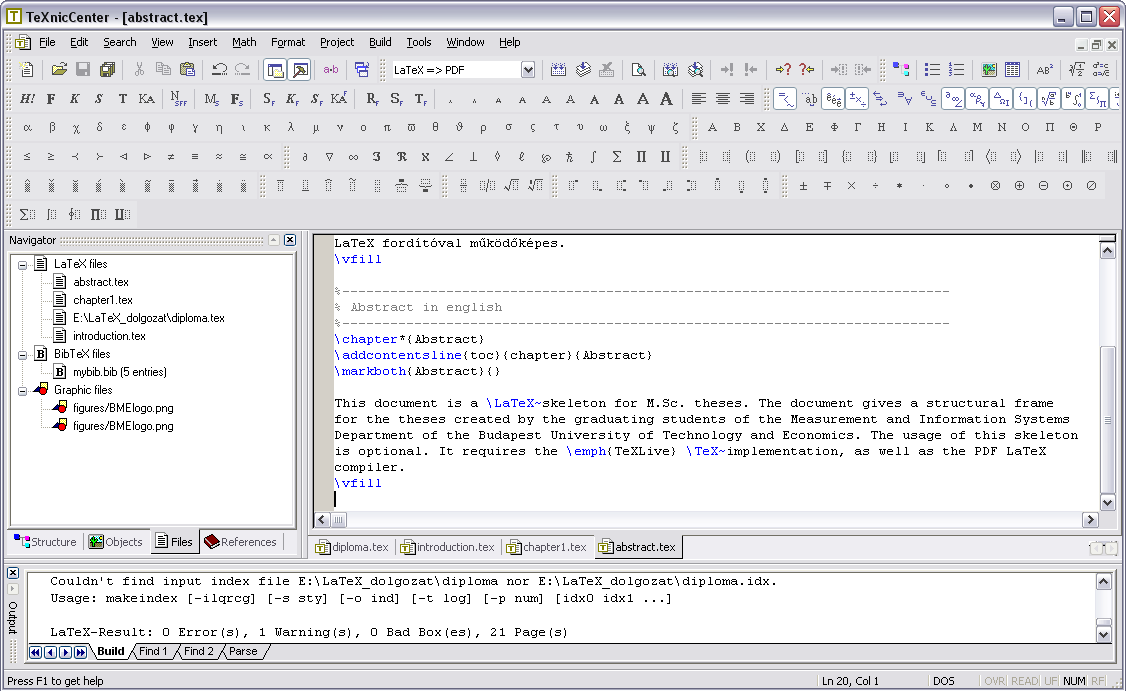
\includegraphics[width=150mm, keepaspectratio]{figures/TeXnicCenter.png}
\caption{A TeXnicCenter Windows alap� \LaTeX-szerkeszt�.} 
\label{fig:TexnicCenter}
\end{figure}

Egy m�sik haszn�lhat� Windows alap� szerkeszt�program a LEd (LaTeX Editor,\\\url{http://www.latexeditor.org/}), a TeXnicCenter azonban stabilabb, gyorsabb, �s jobban haszn�lhat�.

%----------------------------------------------------------------------------
\section{A dokumentum leford�t�sa Windows alatt}
%----------------------------------------------------------------------------
A TeXnicCenter �s a LEd kiz�r�lag szerkeszt�program (b�r az ut�bbiban DVI-n�zeget� is van), �gy a dokumentum ford�t�s�hoz sz�ks�ges eszk�z�ket nem tartalmazza. Windows alatt alapvet�en k�t lehet�s�g k�z�l �rdemes v�lasztani: MiKTeX (\url{http://miktex.org/}) �s TeXLive (\url{http://www.tug.org/texlive/}) programcsomag. Az ut�bbi m�k�dik Mac OS X, GNU/Linux alatt �s Unix-sz�rmaz�kokon is. A MiKTeX egy alapcsomag telep�t�se ut�n mindig let�lti a haszn�lt funkci�khoz sz�ks�ges, de lok�lisan hi�nyz� \TeX-csomagokat, m�g a TeXLive DVD ISO verz�ban f�rhet� hozz�. Ez a dokumentum TeXLive 2008 programcsomag seg�ts�g�vel fordult, amelynek DVD ISO verzi�ja a megadott oldalr�l let�lthet�. A sablon leford�t�s�hoz a disztrib�ci�ban szerepl� \verb+magyar.ldf+ f�jlt a \verb+http://www.math.bme.hu/latex/+ v�ltozatra kell cser�lni, vagy az ut�bbi v�ltozatot be kell m�solni a projekt-k�nyvt�rba (ahogy ezt meg is tett�k a sablonban) k�l�nben anom�li�k tapasztalhat�k a dokumentumban (pl. az �bra- �s t�bl�zat-al��r�sok form�tuma nem a be�ll�tott lesz, vagy bizonyos oldalakon megjelenik alap�telmez�sben egy fejl�c). A TeXLive 2008-at m�g nem kell k�l�n telep�teni a g�pre, elegend� DVD-r�l (vagy az ISO f�jlb�l k�zvetlen�l, pl. DaemonTools-szal) haszn�lni. 

A \TeX-eszk�z�ket tartalmaz� programcsomag bin�risainak el�r�si �tj�t minden esetben be kell �ll�tani a szerkeszt�programban, p�ld�ul TeXnicCenter eset�n legegyszer�bben a \verb+Build / Define output profiles...+ men�ponttal el�h�vott dial�gusablakban a \verb+Wizard...+ gombra kattintva tehetj�k ezt meg.

A PDF-\LaTeX~haszn�lata eset�n a gener�lt dokumentum k�zvetlen�l PDF-form�tumban �ll rendelkez�sre. Amennyiben a PDF-f�jl egy PDF-n�z�ben (pl. Adobe Acrobat Reader vagy Foxit PDF Reader) meg van nyitva, akkor a f�jlle�r�t a PDF-n�z� program tipikusan lefoglalja. Ilyen esetben a dokumentum �jraford�t�sa hiba�zenettel kil�p. Ha bez�rjuk �s �jra megnyitjuk a PDF dokumentumot, akkor pedig a PDF-n�z�k t�bbs�ge az els� oldalon nyitja meg a dokumentumot, nem a legut�bb olvasott oldalon. Ezzel szemben p�ld�ul az egyszer� �s ingyenes \textcolor{blue}{Sumatra PDF} nev� program k�pes arra, hogy a megnyitott dokumentum megv�ltoz�s�t detekt�lja, �s friss�tse a n�zetet az aktu�lis oldal megtart�s�val.

%----------------------------------------------------------------------------
\section{Eszk�z�k Linuxhoz}
%----------------------------------------------------------------------------
Linux oper�ci�s rendszer alatt is rengeteg szerkeszt�program van, pl. a KDE alap� Kile j�l haszn�lhat�. Ez ingyenesen let�lthet�, vagy �ppens�ggel az adott Linux-disztrib�ci� eleve tartalmazza, ahogyan a dokumentum ford�t�s�hoz sz�ks�ges csomagokat is. Az Ubuntu Linux disztrib�ci�k alatt p�ld�ul legt�bbsz�r a \verb+texlive-base+ csomag telep�t�s�vel haszn�lhat�k a \LaTeX-eszk�z�k.

%----------------------------------------------------------------------------
\chapter{A dolgozat formai kivitele}
%----------------------------------------------------------------------------
Az itt tal�lhat� inform�ci�k egy r�sze a BME VIK Hallgat�i K�pviselet �ltal k�sz�tett ,,Utols� f�l�v a villanykaron'' c. munk�b�l lett kis v�ltoztat�sokkal �temelve. Az eredeti dokumentum az al�bbi linken �rhet� el: \url{http://vik-hk.bme.hu/diplomafelev-howto-2009}.

%----------------------------------------------------------------------------
\section{A dolgozat kim�rete}
%----------------------------------------------------------------------------
A minim�lis 50, az optim�lis kim�ret 60-70 oldal (f�ggel�kkel egy�tt). A b�r�l�k �s a z�r�vizsga bizotts�g sem szereti kifejezetten a t�l hossz� dolgozatokat, �gy a brutt� 90 oldalt m�r nem �rdemes t�lsz�rnyalni. Egy�bk�nt f�ggetlen�l a dolgozat kim�ret�t�l, ha a dolgozat nem �rdekfesz�t�, akkor az olvas� m�r az elej�n a v�g�t fogja v�rni. �rdemes z�rt, �nmag�ban is �rthet� m�vet alkotni.

%----------------------------------------------------------------------------
\section{A dolgozat nyelve}
%----------------------------------------------------------------------------
Mivel Magyarorsz�gon a hivatalos nyelv a magyar, ez�rt alap�rtelmez�sben magyarul kell meg�rni a dolgozatot. Aki k�lf�ldi posztgradu�lis k�pz�sben akar r�szt venni, nemzetk�zi szint� tudom�nyos kutat�st szeretne v�gezni, vagy multinacion�lis c�gn�l akar elhelyezkedni, annak c�lszer� angolul meg�rnia diplomadolgozat�t. Miel�tt a hallgat� az angol nyelv� verzi� mellett d�nt, er�sen aj�nlott m�rlegelni, hogy ez mennyi t�bbletmunk�t fog a hallgat�nak jelenteni fogalmaz�s �s nyelvhelyess�g ter�n, valamint - nem utols� sorban - hogy ez mennyi t�bbletmunk�t fog jelenteni a konzulens illetve b�r�l� sz�m�ra. Egy nehezen olvashat�, netal�n �rthetetlen sz�veg teher minden j�t�kos sz�m�ra.

%----------------------------------------------------------------------------
\section{A dokumentum nyomdatechnikai kivitele}
%----------------------------------------------------------------------------
A dolgozatot A4-es feh�r lapra nyomtatva, 2,5 centim�teres marg�val (+1~cm k�t�sbeni), 11-12 pontos bet�m�rettel, talpas bet�t�pussal �s m�sfeles sork�zzel c�lszer� elk�sz�teni.



%----------------------------------------------------------------------------
\chapter{A \LaTeX-sablon haszn�lata}
%----------------------------------------------------------------------------
Ebben a fejezetben r�viden, implicit m�don bemutatjuk a sablon haszn�lat�nak m�dj�t, ami azt jelenti, hogy sablon haszn�lata ennek a dokumentumnak a forr�sk�dj�t tanulm�nyozva v�lik teljesen vil�goss�. Amennyiben a szoftver-keretrendszer telep�tve van, a sablon alkalmaz�sa �s a dolgozat szerkeszt�se \LaTeX-ben a sablon seg�ts�g�vel tapasztalataink szerint j�val hat�konyabb, mint egy WYSWYG (\emph{What You See is What You Get}) t�pus� sz�vegszerkeszt� eset�n (pl. Microsoft Word, OpenOffice).

%----------------------------------------------------------------------------
\section{C�mk�k �s hivatkoz�sok}
%----------------------------------------------------------------------------
A \LaTeX~dokumentumban c�mk�ket (\verb+\label+) rendelhet�nk �br�khoz, t�bl�zatokhoz, fejezetekhez, list�khoz, k�pletekhez stb. Ezekre a dokumentum b�rmely r�sz�ben hivatkozhatunk, a hivatkoz�sok automatikusan felold�sra ker�lnek.

A sablonban makr�kat defini�ltunk a hivatkoz�sok megk�nny�t�s�hez. Ennek megfelel�en minden �bra (\emph{figure}) c�mk�je \verb+fig:+ kulcssz�val kezd�dik, m�g minden t�bl�zat (\emph{table}), k�plet (\emph{equation}), fejezet (\emph{section}) �s lista (\emph{listing}) rendre a \verb+tab:+, \verb+eq:+, \verb+sect:+ �s \verb+listing:+ kulcssz�val kezd�dik, �s a kulcsszavak ut�n tetsz�legesen v�lasztott c�mke haszn�lhat�. Ha ezt a konvenci�t betartjuk, akkor az el�bbi objektumok sz�m�ra rendre a \verb+\figref+, \verb+\tabref+, \verb+\eqref+, \verb+\sectref+ �s \verb+\listref+ makr�kkal hivatkozhatunk. A makr�k param�tere a c�mke, amelyre hivatkozunk (a kulcssz� n�lk�l). Az �sszes eml�tett hivatkoz�st�pus, bele�rtve az \verb+\url+ kulcssz�val bevezetett web-hivatkoz�sokat is a  \verb+hyperref+\footnote{Seg�ts�g�vel a dokumentumban megjelen� hivatkoz�sok nem csak dinamikuss� v�lnak, de sz�nezhet�k is, b�vebbet err�l a csomag dokument�ci�j�ban tal�lunk. Ez egy�ttal egy p�lda l�bjegyzet �r�s�ra.} csomagnak k�sz�nhet�en akt�vak a legt�bb PDF-n�zeget�ben, r�juk kattintva a dokumentum megfelel� oldal�ra ugrik a PDF-n�z� vagy a megfelel� linket megnyitja az alap�rtelmezett b�ng�sz�vel. A \verb+hyperref+ csomag a kimeneti PDF-dokumentumba k�nyvjelz�ket is k�sz�t a tartalomjegyz�kb�l. Ez egy szint�n akt�v tartalomjegyz�k, amelynek elemeire kattintva a n�zeget� behozza a kiv�lasztott fejezetet.

%----------------------------------------------------------------------------
\section{�br�k �s t�bl�zatok}
%----------------------------------------------------------------------------
A k�peket PDFLaTeX eset�n a vesztes�gmentes PNG, valamint a vesztes�ges JPEG form�tumban �rdemes elmenteni. Az EPS (PostScript) vektorgrafikus k�pform�tum beilleszt�s�t a PDFLatex k�zvetlen�l nem t�mogatja. Ehelyett egy lehet�s�g 200 dpi, vagy ann�l nagyobb felbont�sban raszteriz�lni a k�pet, �s PNG form�tumban elmenteni. Az egyes k�pek m�rete �ltal�ban nem, de sok k�p eset�n a dokumentum �sszm�rete �gy m�r szignifik�ns is lehet. A dokumentumban felhaszn�lt k�pf�jlokat a dokumentum forr�sa mellett �rdemes tartani, archiv�lni, mivel ezek hi�ny�ban a dokumentum nem fordul �jra. Ha lehet, a vektorgrafikus k�peket vektorgrafikus form�tumban is �rdemes elmenteni az �jrafelhaszn�lhat�s�g (az �tszerkeszthet�s�g) �rdek�ben.

Kapcsol�si rajzok legt�bbsz�r kim�solhat�k egy vektorgrafikus programba (pl. CorelDraw) �s onnan nagyobb felbont�ssal raszteriz�lva kimenthat�k PNG form�tumban. Ugyanakkor kiv�l� �br�k k�sz�thet�k Microsoft Visio vagy hasonl� program haszn�lat�val is: Visio-b�l az �br�k k�zvetlen�l PNG-be is menthet�k.

Lehet�s�geink Matlab �br�k eset�n:
\begin{itemize}
	\item K�perny�lop�s (\emph{screenshot}) is elfogadhat� min�s�g� lehet a dokumentumban, de �ltal�ban jobb felbont�st is el lehet �rni m�s m�dszerrel.
	\item A Matlab �br�t a \verb+File/Save As+ opci�val lementhetj�k PNG form�tumban (ugyanaz itt is �rv�nyes, mint kor�bban, ez�rt nem javasoljuk).
	\item A Matlab �br�t az \verb+Edit/Copy figure+ opci�val kim�solhatjuk egy vektorgrafikus programba is �s onnan nagyobb felbont�ssal raszteriz�lva kimenthatj�k PNG form�tumban (nem javasolt).
	\item Javasolt megold�s: az �br�t a \verb+File/Save As+ opci�val EPS \emph{vektorgrafikus} form�tumban elmentj�k, PDF-be konvert�lva beillesztj�k a dolgozatba.
\end{itemize}
Az EPS k�p az \verb+epstopdf+ programmal\footnote{a kor�bban eml�tett \LaTeX-disztrib�ci�kban megtal�lhat�} konvert�lhat� PDF form�tumba. C�lszer� egy batch-f�jlt k�sz�teni az �sszes EPS �bra leford�t�s�ra az al�bbi m�don (ez Windows alatt m�k�dik).
\begin{lstlisting}[frame=single,float=!ht]
@echo off
for %%j in (*.eps) do (
echo converting file "%%j"
epstopdf "%%j"
)
echo done .
\end{lstlisting}

Egy ilyen parancsf�jlt (\verb+convert.cmd+) elhelyezt�k a sablon \verb+figures\eps+ k�nyvt�r�ba, �gy a felhaszn�l�nak csak annyi a dolga, hogy a \verb+figures\eps+ k�nyvt�rba kimenti az EPS form�tum� vektorgrafikus k�pet, majd lefuttatja a \verb+convert.cmd+ parancsf�jlt, ami PDF-be konvert�lja az EPS f�jlt.

Ezek ut�n a PDF-�br�t ugyan�gy lehet a dokumentumba beilleszteni, mint a PNG-t vagy a JPEG-et. A megold�s el�nye, hogy a leford�tott dokumentumban is vektorgrafikusan t�rol�dik az �bra, �gy a m�rete j�val kisebb, mintha raszteriz�ltuk volna beilleszt�s el�tt. Ez a m�dszer minden -- az EPS form�tumot ismer� -- vektorgrafikus program (pl. CorelDraw) eset�n is haszn�lhat�.

A k�pek beilleszt�s�re az \sectref{LatexTools}. fejezetben mutattunk be p�ld�t (\figref{TexnicCenter}~�bra). Az el�z� mondatban egy�ttal az automatikusan felold�d� �brahivatkoz�sra is l�thatunk p�ld�t. T�bb k�pf�jlt is beilleszthet�nk egyetlen �br�ba. Az egyes k�pek k�z�tti horizont�lis �s vertik�lis marg�t metrikusan szab�lyozhatjuk (\figref{HVSpaces}~�bra). Az �br�k elhelyez�s�t sz�mtalan tipogr�fiai szab�ly egyidej� teljes�t�s�vel a ford�t� maga v�gzi, a dokumentum �r�ja csak preferenci�it jelezheti a ford�t� fel� (olykor ez bossz�s�got is okozhat, ilyenkor pl. a k�p m�ret�vel lehet j�tszani).

\begin{figure}[!ht]
\centering
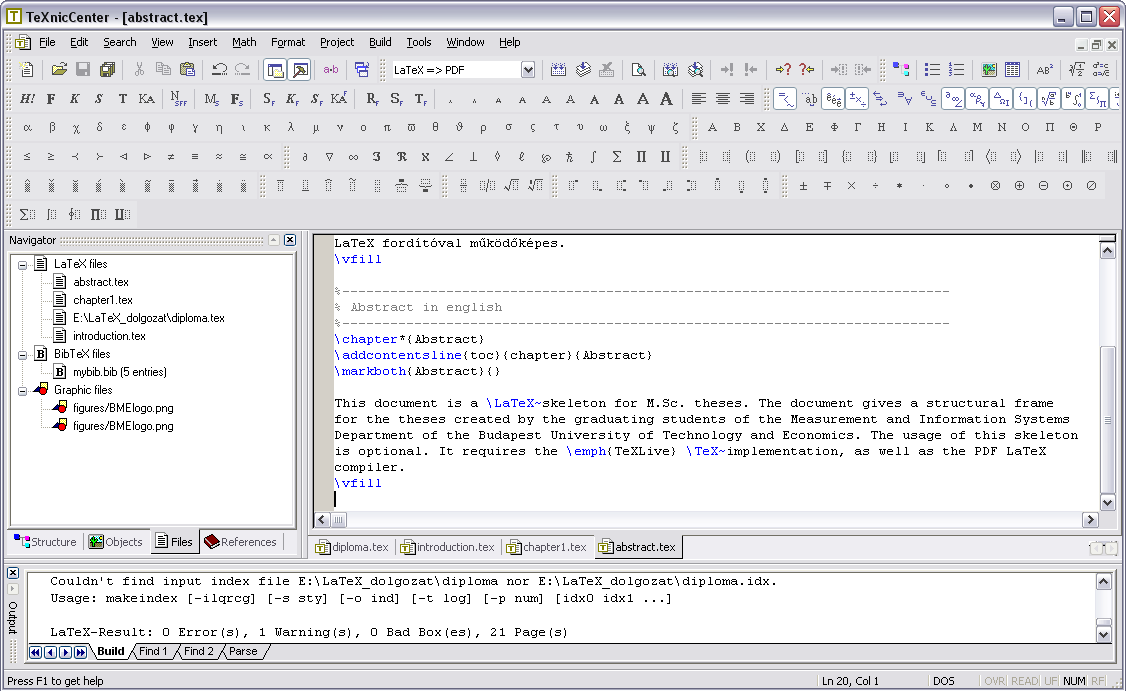
\includegraphics[width=67mm, keepaspectratio]{figures/TeXnicCenter.png}\hspace{1cm}
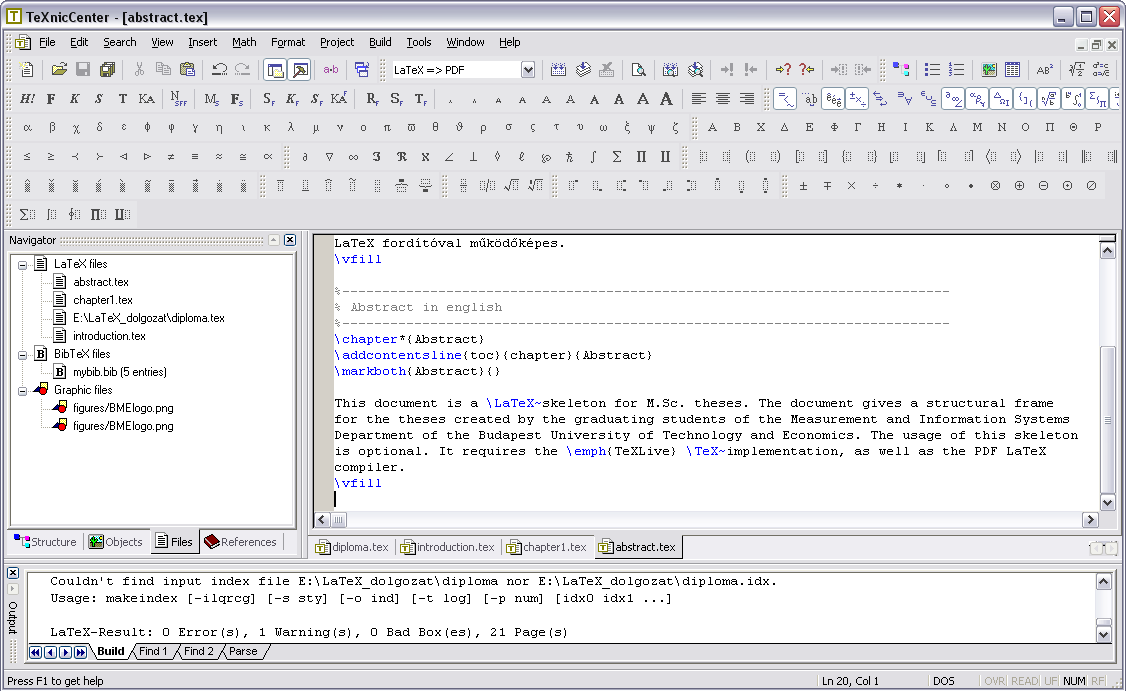
\includegraphics[width=67mm, keepaspectratio]{figures/TeXnicCenter.png}\\\vspace{5mm}
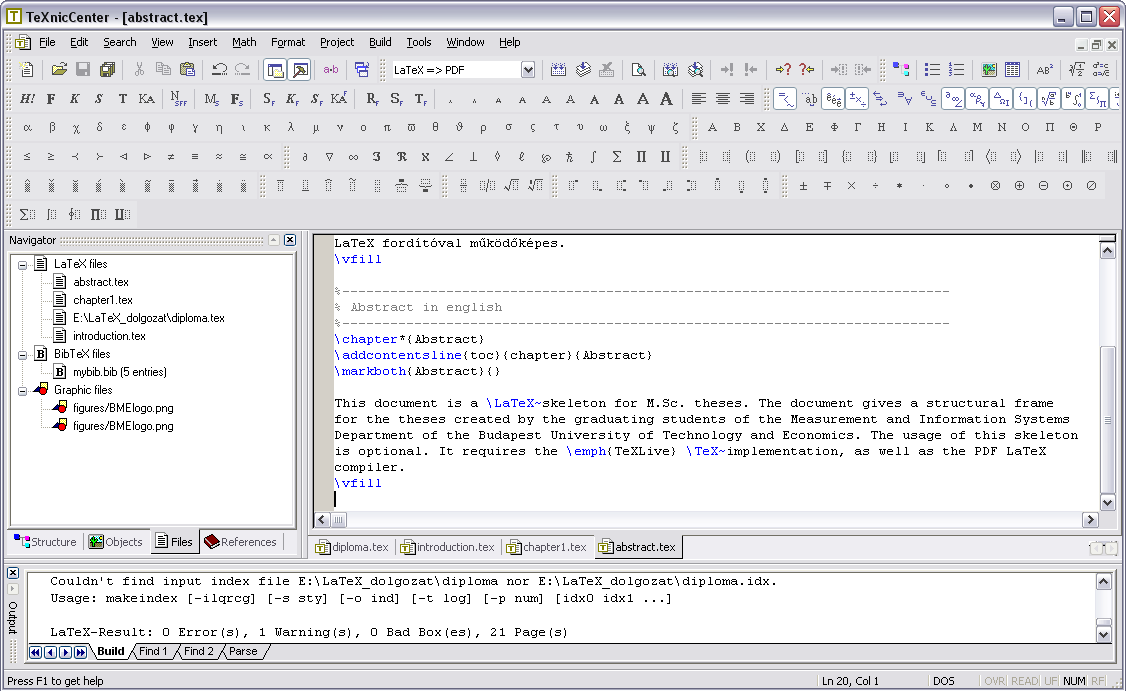
\includegraphics[width=67mm, keepaspectratio]{figures/TeXnicCenter.png}\hspace{1cm}
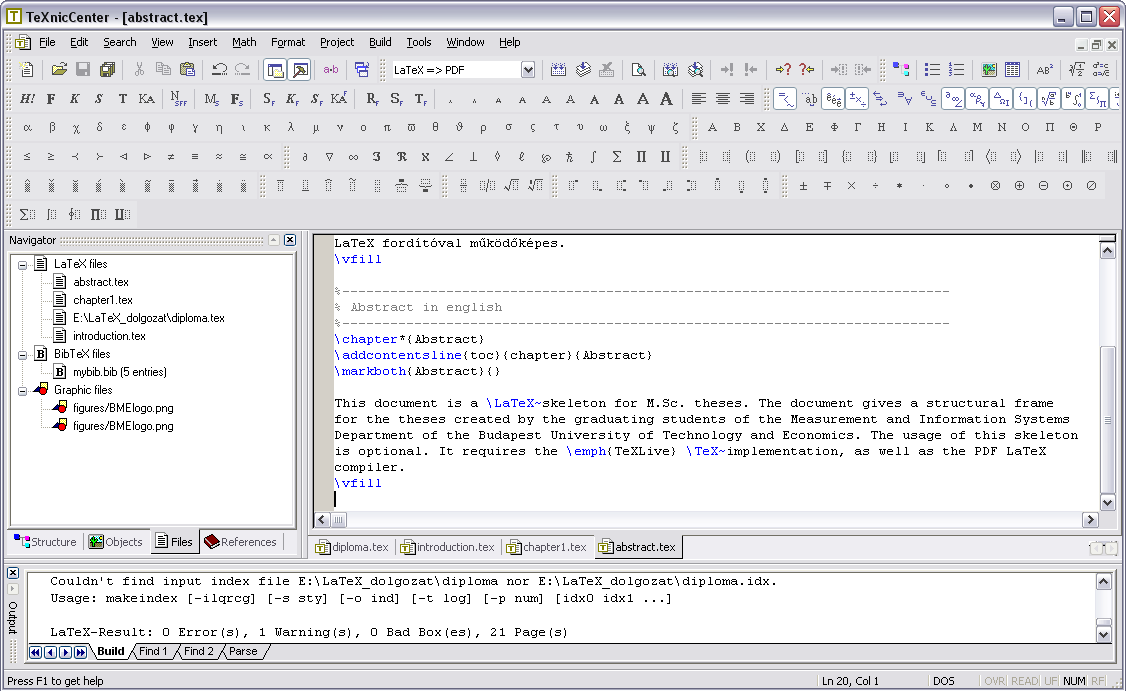
\includegraphics[width=67mm, keepaspectratio]{figures/TeXnicCenter.png}
\caption{T�bb k�pf�jl beilleszt�se eset�n t�rk�z�ket is �rdemes haszn�lni.} 
\label{fig:HVSpaces}
\end{figure}

A t�bl�zatok haszn�lat�ra a \tabref{TabularExample}~t�bl�zat mutat p�ld�t.
A t�bl�zat c�mk�je nem v�letlen�l ker�lt a t�bl�zat f�l�, ez a szokv�nyos.
\begin{table}[ht]
	\footnotesize
	\centering
	\caption{Az �rajel-gener�tor chip �rajel-kimenetei.} \label{tab:SysClocks}
	\begin{tabular}{ | l | c | c |}
	\hline
	�rajel & Frekvencia & C�l pin \\ \hline
	CLKA & 100 MHz & FPGA CLK0\\
	CLKB & 48 MHz  & FPGA CLK1\\
	CLKC & 20 MHz  & Processzor\\
	CLKD & 25 MHz  & Ethernet chip \\
	CLKE & 72 MHz  & FPGA CLK2\\
	XBUF & 20 MHz  & FPGA CLK3\\
	\hline
	\end{tabular}
	\label{tab:TabularExample}
\end{table}


%----------------------------------------------------------------------------
\section{Felsorol�sok �s list�k}
%----------------------------------------------------------------------------
Sz�mozatlan felsorol�sra mutat p�ld�t a jelenlegi bekezd�s:
\begin{itemize}
	\item \emph{els� bajusz:} ide lehetne �rni az els� elem kifej�s�t,
	\item \emph{m�sodik bajusz:} ide lehetne �rni a m�sodik elem kifej�s�t,
	\item \emph{ez meg egy szak�ll:} ide lehetne �rni a harmadik elem kifej�s�t.
\end{itemize}

Sz�mozott felsorol�st is k�sz�thet�nk az al�bbi m�don:
\begin{enumerate}
	\item \emph{els� bajusz:} ide lehetne �rni az els� elem kifej�s�t, �s ez a kifejt�s �gy n�z ki, ha t�bb sorosra sikeredik,
	\item \emph{m�sodik bajusz:} ide lehetne �rni a m�sodik elem kifej�s�t,
	\item \emph{ez meg egy szak�ll:} ide lehetne �rni a harmadik elem kifej�s�t.
\end{enumerate}
A felsorol�sokban sorok v�g�n vessz�, az utols� sor v�g�n pedig pont a szok�sos �r�sjel. Ez al�l kiv�telt k�pezhet, ha az egyes elemek t�bb teljes mondatot tartalmaznak.

List�kban a dolgozat sz�veg�t�l elk�l�n�tend� k�dr�szleteket, programsorokat, pszeudo-k�dokat jelen�thet�nk meg (\listref{Example}~lista). 
\begin{lstlisting}[frame=single,float=!ht,caption=A fenti sz�mozott felsorol�s \LaTeX- forr�sk�dja, label=listing:Example]
\begin{enumerate}
	\item \emph{els� bajusz:} ide lehetne �rni az els� elem kifej�s�t, 
	�s ez a kifejt�s �gy n�z ki, ha t�bb sorosra sikeredik,
	\item \emph{m�sodik bajusz:} ide lehetne �rni a m�sodik elem kifej�s�t,
	\item \emph{ez meg egy szak�ll:} ide lehetne �rni a harmadik elem kifej�s�t.
\end{enumerate}
\end{lstlisting}
A lista keret�t, h�tt�rsz�n�t, eg�sz st�lus�t megv�laszthatjuk. R�ad�sul k�l�nf�le programnyelveket �s a nyelveken bel�l kulcsszavakat is defini�lhatunk, ha sz�ks�ges. Err�l b�vebbet a \verb+listings+ csomag hivatalos le�r�s�ban tal�lhatunk.

%----------------------------------------------------------------------------
\section{K�pletek}
%----------------------------------------------------------------------------
Ha egy formula nem t�ls�gosan hossz�, �s nem akarjuk hivatkozni a sz�vegb�l, mint p�ld�ul a $e^{i\pi}+1=0$ k�plet, \emph{sz�vegk�zi k�pletk�nt} szok�s le�rni. Csak, hogy m�sik p�ld�t is l�ssunk, az $U_i=-d\Phi/dt$ Faraday-t�rv�ny a $\rot E=-\frac{dB}{dt}$ differenci�lis alakban adott Maxwell-egyenlet fel�letre vett integr�lj�b�l vezethet� le. L�that�, hogy a \LaTeX-ford�t� a sork�z�ket betartja, �gy a sz�veg szed�se eszt�tikus marad sz�vegk�zi k�pletek haszn�lata eset�n is.

K�pletek eset�n az �ltal�nos konvenci�, hogy a kisbet�k skal�rt, a kis f�lk�v�r bet�k ($\mathbf{v}$) oszlopvektort -- �s ennek megfelel�en $\mathbf{v}^T$ sorvektort -- a kapit�lis f�lk�v�r bet�k ($\mathbf{V}$) m�trixot jel�lnek. Ha ett�l el szeretn�nk t�rni, akkor az alkalmazni k�v�nt jel�l�sm�dot c�lszer� k�l�n alfejezetben defini�lni. Ennek megfelel�en, amennyiben $\mathbf{y}$ jel�li a m�r�sek vektor�t, $\mathbf{\vartheta}$ a param�terek vektor�t �s $\hat{\mathbf{y}}=\mathbf{X}\vartheta$ a param�terekben line�ris modellt, akkor a \emph{Least-Squares} �rtelemben optim�lis param�terbecsl� $\hat{\mathbf{\vartheta}}_{LS}=(\mathbf{X}^T\mathbf{X})^{-1}\mathbf{X}^T\mathbf{y}$ lesz.

Emellett kiemelt, sorsz�mozott k�pleteket is megadhatunk, enn�l az \verb+equation+ �s a \verb+eqnarray+ k�rnyezetek helyett a korszer�bb \verb+align+ k�rnyezet alkalmaz�s�t javasoljuk (t�bb okb�l, k�l�nf�le probl�m�k elker�l�se v�gett, amelyekre most nem t�r�nk ki). Teh�t
\begin{align}
\dot{\mathbf{x}}&=\mathbf{A}\mathbf{x}+\mathbf{B}\mathbf{u},\\
\mathbf{y}&=\mathbf{C}\mathbf{x},
\end{align}
ahol $\mathbf{x}$ az �llapotvektor, $\mathbf{y}$ a m�r�sek vektora �s $\mathbf{A}$, $\mathbf{B}$ �s $\mathbf{C}$ a rendszert le�r� param�term�trixok. Figyelj�k meg, hogy a k�t egyenletben az egyenl�s�gjelek egym�shoz igaz�tva jelennek meg, mivel a mindkett�t az \& karakter el�zi meg a k�dban. Lehet�s�g van sz�mozatlan kiemelt k�plet haszn�lat�ra is, p�ld�ul
\begin{align}
\dot{\mathbf{x}}&=\mathbf{A}\mathbf{x}+\mathbf{B}\mathbf{u},\nonumber\\
\mathbf{y}&=\mathbf{C}\mathbf{x}\nonumber.
\end{align}
M�trixok fel�r�s�ra az $\mathbf{A}\mathbf{x}=\mathbf{b}$ inhomog�n line�ris egyenlet r�szletes kifejt�s�vel mutatunk p�ld�t:
\begin{align}
\begin{bmatrix}
a_{11} & a_{12} & \dots & a_{1n}\\
a_{21} & a_{22} & \dots & a_{2n}\\
\vdots & \vdots & \ddots & \vdots\\
a_{m1} & a_{m2} & \dots & a_{mn}
\end{bmatrix}
\begin{pmatrix}x_1\\x_2\\\vdots\\x_n\end{pmatrix}=
\begin{pmatrix}b_1\\b_2\\\vdots\\b_m\end{pmatrix}.
\end{align}
A \verb+\frac+ utas�t�s hat�konys�g�t egy �ltal�nos m�sodfok� tag �tviteli f�ggv�ny�n kereszt�l mutatjuk be, azaz
\begin{align}
W(s)=\frac{A}{1+2T\xi s+s^2T^2}.
\end{align}
A matematikai m�d minden szimb�lum�nak �s k�pess�g�nek a bemutat�s�ra term�szetesen itt nincs lehet�s�g, de gyors referenciak�nt hat�konyan haszn�lhat�k a k�vetkez� linkek:\\
\indent\url{http://www.artofproblemsolving.com/LaTeX/AoPS_L_GuideSym.php},\\
\indent\url{http://www.ctan.org/tex-archive/info/symbols/comprehensive/symbols-a4.pdf},\\
\indent\url{ftp://ftp.ams.org/pub/tex/doc/amsmath/short-math-guide.pdf}.\\
Ez pedig itt egy magyar�zat, hogy mi�rt �rdemes \verb+align+ k�rnyezetet haszn�lni:\\
\indent\url{http://texblog.net/latex-archive/maths/eqnarray-align-environment/}.

%----------------------------------------------------------------------------
\section{Irodalmi hivatkoz�sok}\label{sect:HowtoReference}
%----------------------------------------------------------------------------
Egy \LaTeX dokumentumban az irodalmi hivatkoz�sok defin�ci�j�nak k�t m�dja van. Az egyik a \verb+\thebibliograhy+ k�rnyezet haszn�lata a dokumentum v�g�n, az \verb+\end{document}+ lez�r�s el�tt.
\begin{lstlisting}[frame=single,float=!ht]
\begin{thebibliography}{9}

\bibitem{Lamport94} Leslie Lamport, \emph{\LaTeX: A Document Preparation System}. 
Addison Wesley, Massachusetts, 2nd Edition, 1994.

\end{thebibliography}
\end{lstlisting}

Ezek ut�n a dokumentumban a \verb+\cite{Lamport94}+ utas�t�ssal hivatkozhatunk a forr�sra. A fenti megad�s viszonylag k�tetlen, a szerz� maga form�zza az irodalomjegyz�ket. 

Egy sokkal professzion�lisabb m�dszer a BiB\TeX~haszn�lata, ez�rt ez a sablon is ezt t�mogatja. Ebben az esetben egy k�l�n sz�veges adatb�zisban defini�ljuk a forr�smunk�kat, �s egy k�l�n st�lusf�jl hat�rozza meg az irodalomjegyz�k kin�zet�t. Ez, �sszhangban azzal, hogy k�l�n form�tumkonvenci� hat�rozza meg a foly�irat-, a k�nyv-, a konferenciacikk- stb. hivatkoz�sok kin�zet�t az irodalomjegyz�kben (a sablon haszn�lata eset�n ezzel nem is kell foglalkoznia a hallgat�nak, de az eredm�nyt c�lszer� ellen�rizni). A felhaszn�lt hivatkoz�sok adatb�zisa egy \verb+.bib+ kiterjeszt�s� sz�veges f�jl, amelynek szerkezet�t a \listref{Bibtex} k�dr�szlet demonstr�lja. A forr�smunk�k bevitelekor a sor v�gi vessz�k k�l�n figyelmet ig�nyelnek, mert hi�nyuk a BiB\TeX-ford�t� hiba�zenet�t eredm�nyezi. A forr�smunk�kat t�pus szerinti kulcssz� vezeti be (\verb+@book+ k�nyv, \verb+@inproceedings+ konferenciakiadv�nyban megjelent cikk, \verb+@article+ foly�iratban megjelent cikk, \verb+@techreport+ valamelyik egyetem gondoz�s�ban megjelent m�szaki tanulm�ny, \verb+@manual+ m�szaki dokument�ci� eset�n stb.). Nemcsak a megjelen�s st�lusa, de a k�telez�en megadand� mez�k is t�pusr�l-t�pusra v�ltoznak. Egy j�l haszn�lhat� referencia a \url{http://en.wikipedia.org/wiki/BibTeX} oldalon tal�lhat�.
\begin{lstlisting}[frame=single,float=!ht,caption=P�lda sz�veges irodalomjegyz�k-adatb�zisra BiBTeX haszn�lata eset�n., label=listing:Bibtex]
@BOOK{Wettl04,
  author="Ferenc Wettl and Gyula Mayer and P�ter Szab�",
  title="\LaTeX~k�zik�nyv",
  publisher="Panem K�nyvkiad�",
  year=2004
}
@ARTICLE{Candy86,
  author ="James C. Candy",
  title  ="Decimation for Sigma Delta Modulation",
  journal="{IEEE} Trans.\ on Communications",
  volume =34,
  number =1,
  pages  ="72--76",
  month  =jan,
  year   =1986,
}
@INPROCEEDINGS{Lee87,
  author =       "Wai L. Lee and Charles G. Sodini",
  title =        "A Topology for Higher Order Interpolative Coders",
  booktitle =    "Proc.\ of the IEEE International Symposium on 
  Circuits and Systems",
  year =         1987,
  vol =          2,
  month =        may # "~4--7",
  address =      "Philadelphia, PA, USA",
  pages =        "459--462"
}
@PHDTHESIS{KissPhD,
  author =   "Peter Kiss",
  title =    "Adaptive Digital Compensation of Analog Circuit Imperfections 
  for Cascaded Delta-Sigma Analog-to-Digital Converters",
  school =   "Technical University of Timi\c{s}oara, Romania",
  month =    apr,
  year =     2000
}
@MANUAL{Schreier00,
  author = "Richard Schreier",
  title  = "The Delta-Sigma Toolbox v5.2",
  organization = "Oregon State University",
  year   = 2000,
  month  = jan,
  note   ="\newline URL: http://www.mathworks.com/matlabcentral/fileexchange/"
}
@MISC{DipPortal,
	author="Budapesti {M}�szaki �s {G}azdas�gtudom�nyi {E}gyetem 
	{V}illamosm�rn�ki �s {I}nformatikai {K}ar",
  title="{D}iplomaterv port�l (2011 febru�r 26.)",
  howpublished="\url{http://diplomaterv.vik.bme.hu/}",
}}
\end{lstlisting}

A st�lusf�jl egy \verb+.sty+ kiterjeszt�s� f�jl, de ezzel l�nyeg�ben nem kell foglalkozni, mert vannak be�p�tett st�lusok, amelyek j�l haszn�lhat�k. Ez a sablon a BiB\TeX-et haszn�lja, a hozz� tartoz� adatb�zisf�jl a \verb+mybib.bib+ f�jl. Megfigyelhet�, hogy az irodalomjegyz�ket a dokumentum v�g�re (a \verb+\end{document}+ utas�t�s el�) beillesztett \verb+\bibliography{mybib}+ utas�t�ssal hozhatjuk l�tre, a st�lus�t pedig ugyanitt a  \verb+\bibliographystyle{plain}+ utas�t�ssal adhatjuk meg. Ebben az esetben a \verb+plain+ el�re defini�lt st�lust haszn�ljuk (a sablonban is ezt �ll�tottuk be). A \verb+plain+ st�luson k�v�l term�szetesen sz�mtalan m�s el�re defini�lt st�lus is l�tezik. Mivel a \verb+.bib+ adatb�zisban ezeket megadtuk, a BiB\TeX-ford�t� is meg tudja k�l�nb�ztetni a szerz�t a c�mt�l �s a kiad�t�l, �s ez alapj�n automatikusan gener�l�dik az irodalomjegyz�k a st�lusf�jl �ltal meghat�rozott st�lusban.

Az egyes forr�smunk�kra a sz�vegb�l tov�bbra is a \verb+\cite+ paranccsal tudunk hivatkozni, �gy a \listref{Bibtex} k�dr�szlet eset�n a hivatkoz�sok rendre \verb+\cite{Wettl04}+, \verb+\cite{Candy86}+, \verb+\cite{Lee87}+, \verb+\cite{KissPhD}+, \verb+\cite{Schreirer00}+ �s \verb+\cite{DipPortal}+. Az irodalomjegyz�kben alap�rtelmez�sben csak azok a forr�smunk�k jelennek meg, amelyekre tal�lhat� hivatkoz�s a sz�vegben, �s ez �gy alapvet�en helyes is, hiszen olyan forr�smunk�kat nem illik az irodalomjegyz�kbe �rni, amelyekre nincs hivatkoz�s.

Mivel a ford�t�si folyamat sor�n t�bb l�p�sben old�dnak fel a szimb�lumok, ez�rt gyakran t�bbsz�r (TeXLive �s TeXnicCenter eset�n 2-3-szor) is le kell ford�tani a dokumentumot. Ilyenkor ez els� 1-2 ford�t�s esetleg szimb�lum-felold�sra vonatkoz� figyelmeztet� �zenettel z�rul. Ha hiba�zenettel z�rul b�rmelyik ford�t�s, akkor nincs �rtelme megism�telni, hanem a hib�t kell megkeresni. A \verb+.bib+ f�jl megv�ltoztat�skor sokszor nincs hat�sa a v�ltoztat�snak azonnal, mivel nem mindig fut �jra a BibTeX ford�t�. Ez�rt c�lszer� a v�ltoztat�s ut�n azt manu�lisan is lefuttatni (TeXnicCenter eset�n \verb+Build/BibTeX+).

Hogy a sz�vegbe �gyazott hivatkoz�sok kin�zet�t demonstr�ljuk, itt most sorban meghivatkozzuk a \cite{Wettl04}, \cite{Candy86}, \cite{Lee87}, \cite{KissPhD} �s az \cite{Schreier00} forr�smunk�t, valamint az \cite{DipPortal} weboldalt.

Megjegyzend�, hogy az �kezetes magyar bet�ket is tartalmaz� \verb+.bib+ f�jl az \verb+inputenc+ csomaggal bet�lt�tt \verb+latin2+ bet�k�szlet miatt ford�that�. Ugyanez a \verb+.bib+ f�jl hiba�zenettel fordul egy olyan dokumentumban, ami nem tartalmazza a \verb+\usepackage[latin2]{inputenc}+ sort. Speci�lis ig�ny eset�n az irodalmi adatb�zis �ltal�nosabb �rv�ny�v� tehet�, ha az �kezetes bet�ket speci�lis latex karakterekkel helyettes�tj�k a \verb+.bib+ f�jlban, pl. � helyett \verb+\'{a}+-t vagy � helyett \verb+\H{o}+-t �runk. 

Oldalt�r�s k�vetkezik (ld. forr�s).
\newpage

%----------------------------------------------------------------------------
\section{A dolgozat szerkezete �s a forr�sf�jlok}
%----------------------------------------------------------------------------
A diplomatervsablon (a kari ir�nyelvek szerint) az al�bbi f� fejezetekb�l �ll:
\begin{enumerate}
	\item 1 oldalas \emph{t�j�koztat�} a szakdolgozat/diplomaterv szerkezet�r�l (\verb+guideline.tex+), ami a v�gs� dolgozatb�l t�rlend�,
	\item \emph{feladatki�r�s} (\verb+project.tex+), a dolgozat nyomtatott verz�j�ban ennek a hely�re ker�l a tansz�k �ltal kiadott, a tansz�kvezet� �ltal al��rt feladatki�r�s, a dolgozat elektronikus verzi�j�ba pedig a feladatki�r�s egy�ltal�n ne ker�lj�n bele, azt k�l�n t�lti fel a tansz�k a diplomaterv-honlapra,
	\item \emph{c�moldal} (\verb+titlepage.tex+),
	\item \emph{tartalomjegyz�k} (\verb+diploma.tex+),
	\item a diplomatervez� \emph{nyilatkozat}a az �n�ll� munk�r�l (\verb+declaration.tex+),
	\item 1-2 oldalas tartalmi \emph{�sszefoglal�} magyarul �s angolul, illetve elk�sz�thet� m�g tov�bbi nyelveken is (\verb+abstract.tex+),
	\item \emph{bevezet�s}: a feladat �rtelmez�se, a tervez�s c�lja, a feladat indokolts�ga, a diplomaterv fel�p�t�s�nek r�vid �sszefoglal�sa (\verb+introduction.tex+),
	\item sorsz�mmal ell�tott \emph{fejezetek}: a feladatki�r�s pontos�t�sa �s r�szletes elemz�se, el�zm�nyek (irodalomkutat�s, hasonl� alkot�sok), az ezekb�l levonhat� k�vetkeztet�sek, a tervez�s r�szletes le�r�sa, a d�nt�si lehet�s�gek �rt�kel�se �s a v�lasztott megold�sok indokl�sa, a megtervezett m�szaki alkot�s �rt�kel�se, kritikai elemz�se, tov�bbfejleszt�si lehet�s�gek (\verb+chapter{1,2..n}.tex+),
	\item esetleges \emph{k�sz�netnyilv�n�t�s}ok (\verb+acknowledgement.tex+),
	\item r�szletes �s pontos \emph{irodalomjegyz�k} (ez a sablon eset�ben automatikusan gener�l�dik a \verb+diploma.tex+ f�jlban elhelyezett \verb+\bibliography+ utas�t�s hat�s�ra, a \sectref{HowtoReference}. fejezetben le�rtak szerint),
	\item \emph{f�ggel�kek} (\verb+appendices.tex+).
\end{enumerate}

A sablonban a fejezetek a \verb+diploma.tex+ f�jlba vannak beillesztve \verb+\include+ utas�t�sok seg�ts�g�vel. Lehet�s�g van arra, hogy csak az �ppen szerkeszt�s alatt �ll� \verb+.tex+ f�jlt ford�tsuk le, ezzel ler�vid�tve a ford�t�si folyamatot. Ezt a lehet�s�get az al�bbi k�dr�szlet biztos�tja a \verb+diploma.tex+ f�jlban.
\begin{lstlisting}[frame=single,float=!ht]
\includeonly{
	guideline,%
	project,%
	titlepage,%
	declaration,%
	abstract,%
	introduction,%
	chapter1,%
	chapter2,%
	chapter3,%
	acknowledgement,%
	appendices,%
}
\end{lstlisting}

Ha az al�bbi k�dr�szletben az egyes sorokat a \verb+%+ szimb�lummal kikommentezz�k, akkor a megfelel� \verb+.tex+ f�jl nem fordul le. Az oldalsz�mok �s a tartalomjegy�k term�szetesen csak akkor billennek helyre, ha a teljes dokumentumot leford�tjuk.

%----------------------------------------------------------------------------
\newpage
\section{Alapadatok megad�sa}
%----------------------------------------------------------------------------
A diplomaterv alapadatait (c�m, szerz�, konzulens, konzulens titulusa) a \verb+diploma.tex+ f�jlban lehet megadni az al�bbi k�dr�szlet m�dos�t�s�val.
\begin{lstlisting}[frame=single,float=!ht]
\newcommand{\vikszerzo}{B�dis-Szomor� Andr�s}
\newcommand{\vikkonzulens}{dr.~Konzulens Elem�r}
\newcommand{\vikcim}{Elektronikus terel�k}
\newcommand{\viktanszek}{M�r�stechnika �s Inform�ci�s Rendszerek Tansz�k}
\newcommand{\vikdoktipus}{Diplomaterv}
\newcommand{\vikdepartmentr}{B�dis-Szomor� Andr�s}
\end{lstlisting}

%----------------------------------------------------------------------------
\section{�j fejezet �r�sa}
%----------------------------------------------------------------------------
A f�fejezetek k�l�n \verb+chapter{1..n}.tex+ f�jlban foglalnak helyet. A sablonhoz 3 fejezet k�sz�lt. Tov�bbi f�fejezeteket �gy hozhatunk l�tre, ha �j \verb+chapter{i}.tex+ f�jlt k�sz�t�nk a fejezet sz�m�ra, �s a \verb+diploma.tex+ f�jlban, a \verb+\include+ �s \verb+\includeonly+ utas�t�sok argumentum�ba felvessz�k az �j \verb+.tex+ f�jl nev�t.






%----------------------------------------------------------------------------
\chapter*{K�sz�netnyilv�n�t�s}\addcontentsline{toc}{chapter}{K�sz�netnyilv�n�t�s}
%----------------------------------------------------------------------------

Ez nem k�telez�, ak�r t�r�lhet� is. Ha a szerz� sz�ks�g�t �rzi, itt lehet k�sz�netet nyilv�n�tani azoknak, akik hozz�j�rultak munk�jukkal ahhoz, hogy a hallgat� a szakdolgozatban vagy diplomamunk�ban le�rt feladatokat sikeresen elv�gezze. A konzulensnek val� k�sz�netnyilv�n�t�s sem k�telez�, a konzulensnek hivatalosan is dolga, hogy a hallgat�t konzult�lja.

%\listoffigures\addcontentsline{toc}{chapter}{�br�k jegyz�ke}
%\listoftables\addcontentsline{toc}{chapter}{T�bl�zatok jegyz�ke}

\bibliography{mybib}
\addcontentsline{toc}{chapter}{Irodalomjegyz�k}
\bibliographystyle{plain}

%----------------------------------------------------------------------------
\appendix
%----------------------------------------------------------------------------
\chapter*{F�ggel�k}\addcontentsline{toc}{chapter}{F�ggel�k}
\setcounter{chapter}{6}  % a fofejezet-szamlalo az angol ABC 6. betuje (F) lesz
\setcounter{equation}{0} % a fofejezet-szamlalo az angol ABC 6. betuje (F) lesz
\numberwithin{equation}{section}
\numberwithin{figure}{section}
\numberwithin{lstlisting}{section}
%\numberwithin{tabular}{section}

%----------------------------------------------------------------------------
\section{A TeXnicCenter fel�lete}
%----------------------------------------------------------------------------
\begin{figure}[!ht]
\centering
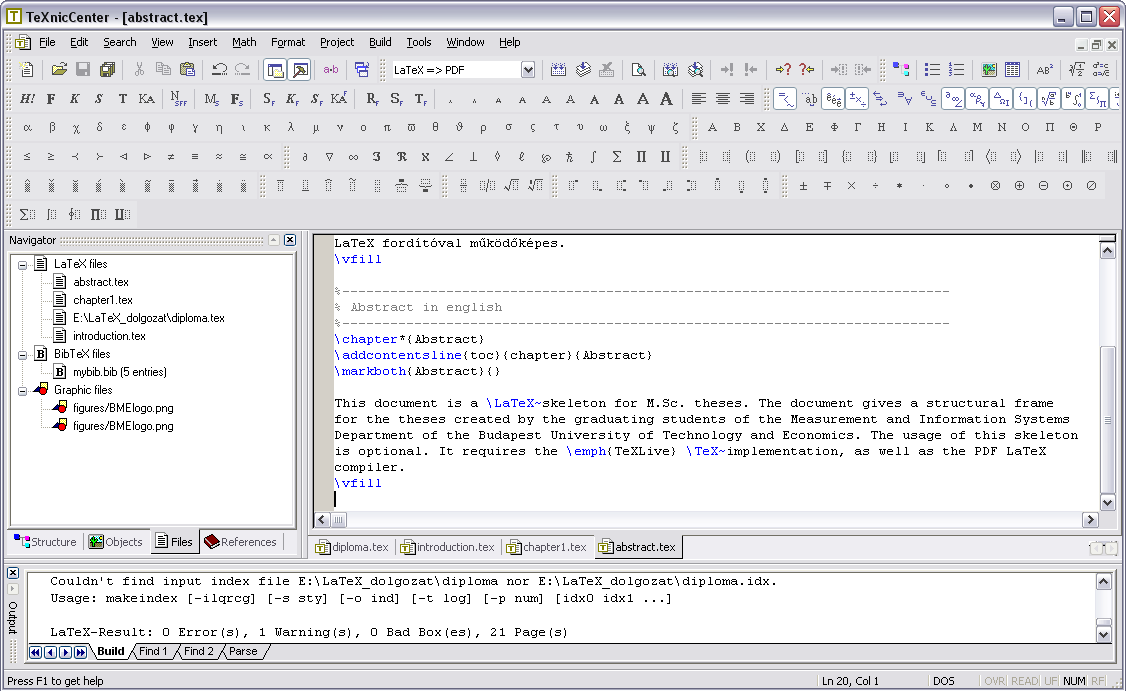
\includegraphics[width=150mm, keepaspectratio]{figures/TeXnicCenter.png}
\caption{A TeXnicCenter Windows alap� \LaTeX-szerkeszt�.} 
\end{figure}

%----------------------------------------------------------------------------
\clearpage\section{V�lasz az ,,�let, a vil�gmindens�g, meg minden'' k�rd�s�re}
%----------------------------------------------------------------------------
A Pitagorasz-t�telb�l levezetve
\begin{align}
c^2=a^2+b^2=42.
\end{align}
A Faraday-indukci�s t�rv�nyb�l levezetve
\begin{align}
\rot E=-\frac{dB}{dt}\hspace{1cm}\longrightarrow \hspace{1cm}
U_i=\oint\limits_\mathbf{L}{\mathbf{E}\mathbf{dl}}=-\frac{d}{dt}\int\limits_A{\mathbf{B}\mathbf{da}}=42.
\end{align}







\label{page:last}
\end{document}
